\section{Question 1}
$$
G(s) = \exp(-\tau s), \quad \tau > 0
$$

$$
\angle G(j\omega) = -\tau \omega
$$
$$
\left\vert G(j\omega) \right\vert = 1 \to 20\log(\left\vert G(j\omega) \right\vert) = 0
$$
\begin{figure}[H]
	\caption{Bode digram using MATLAB ($\tau = 1$)}
	\centering
	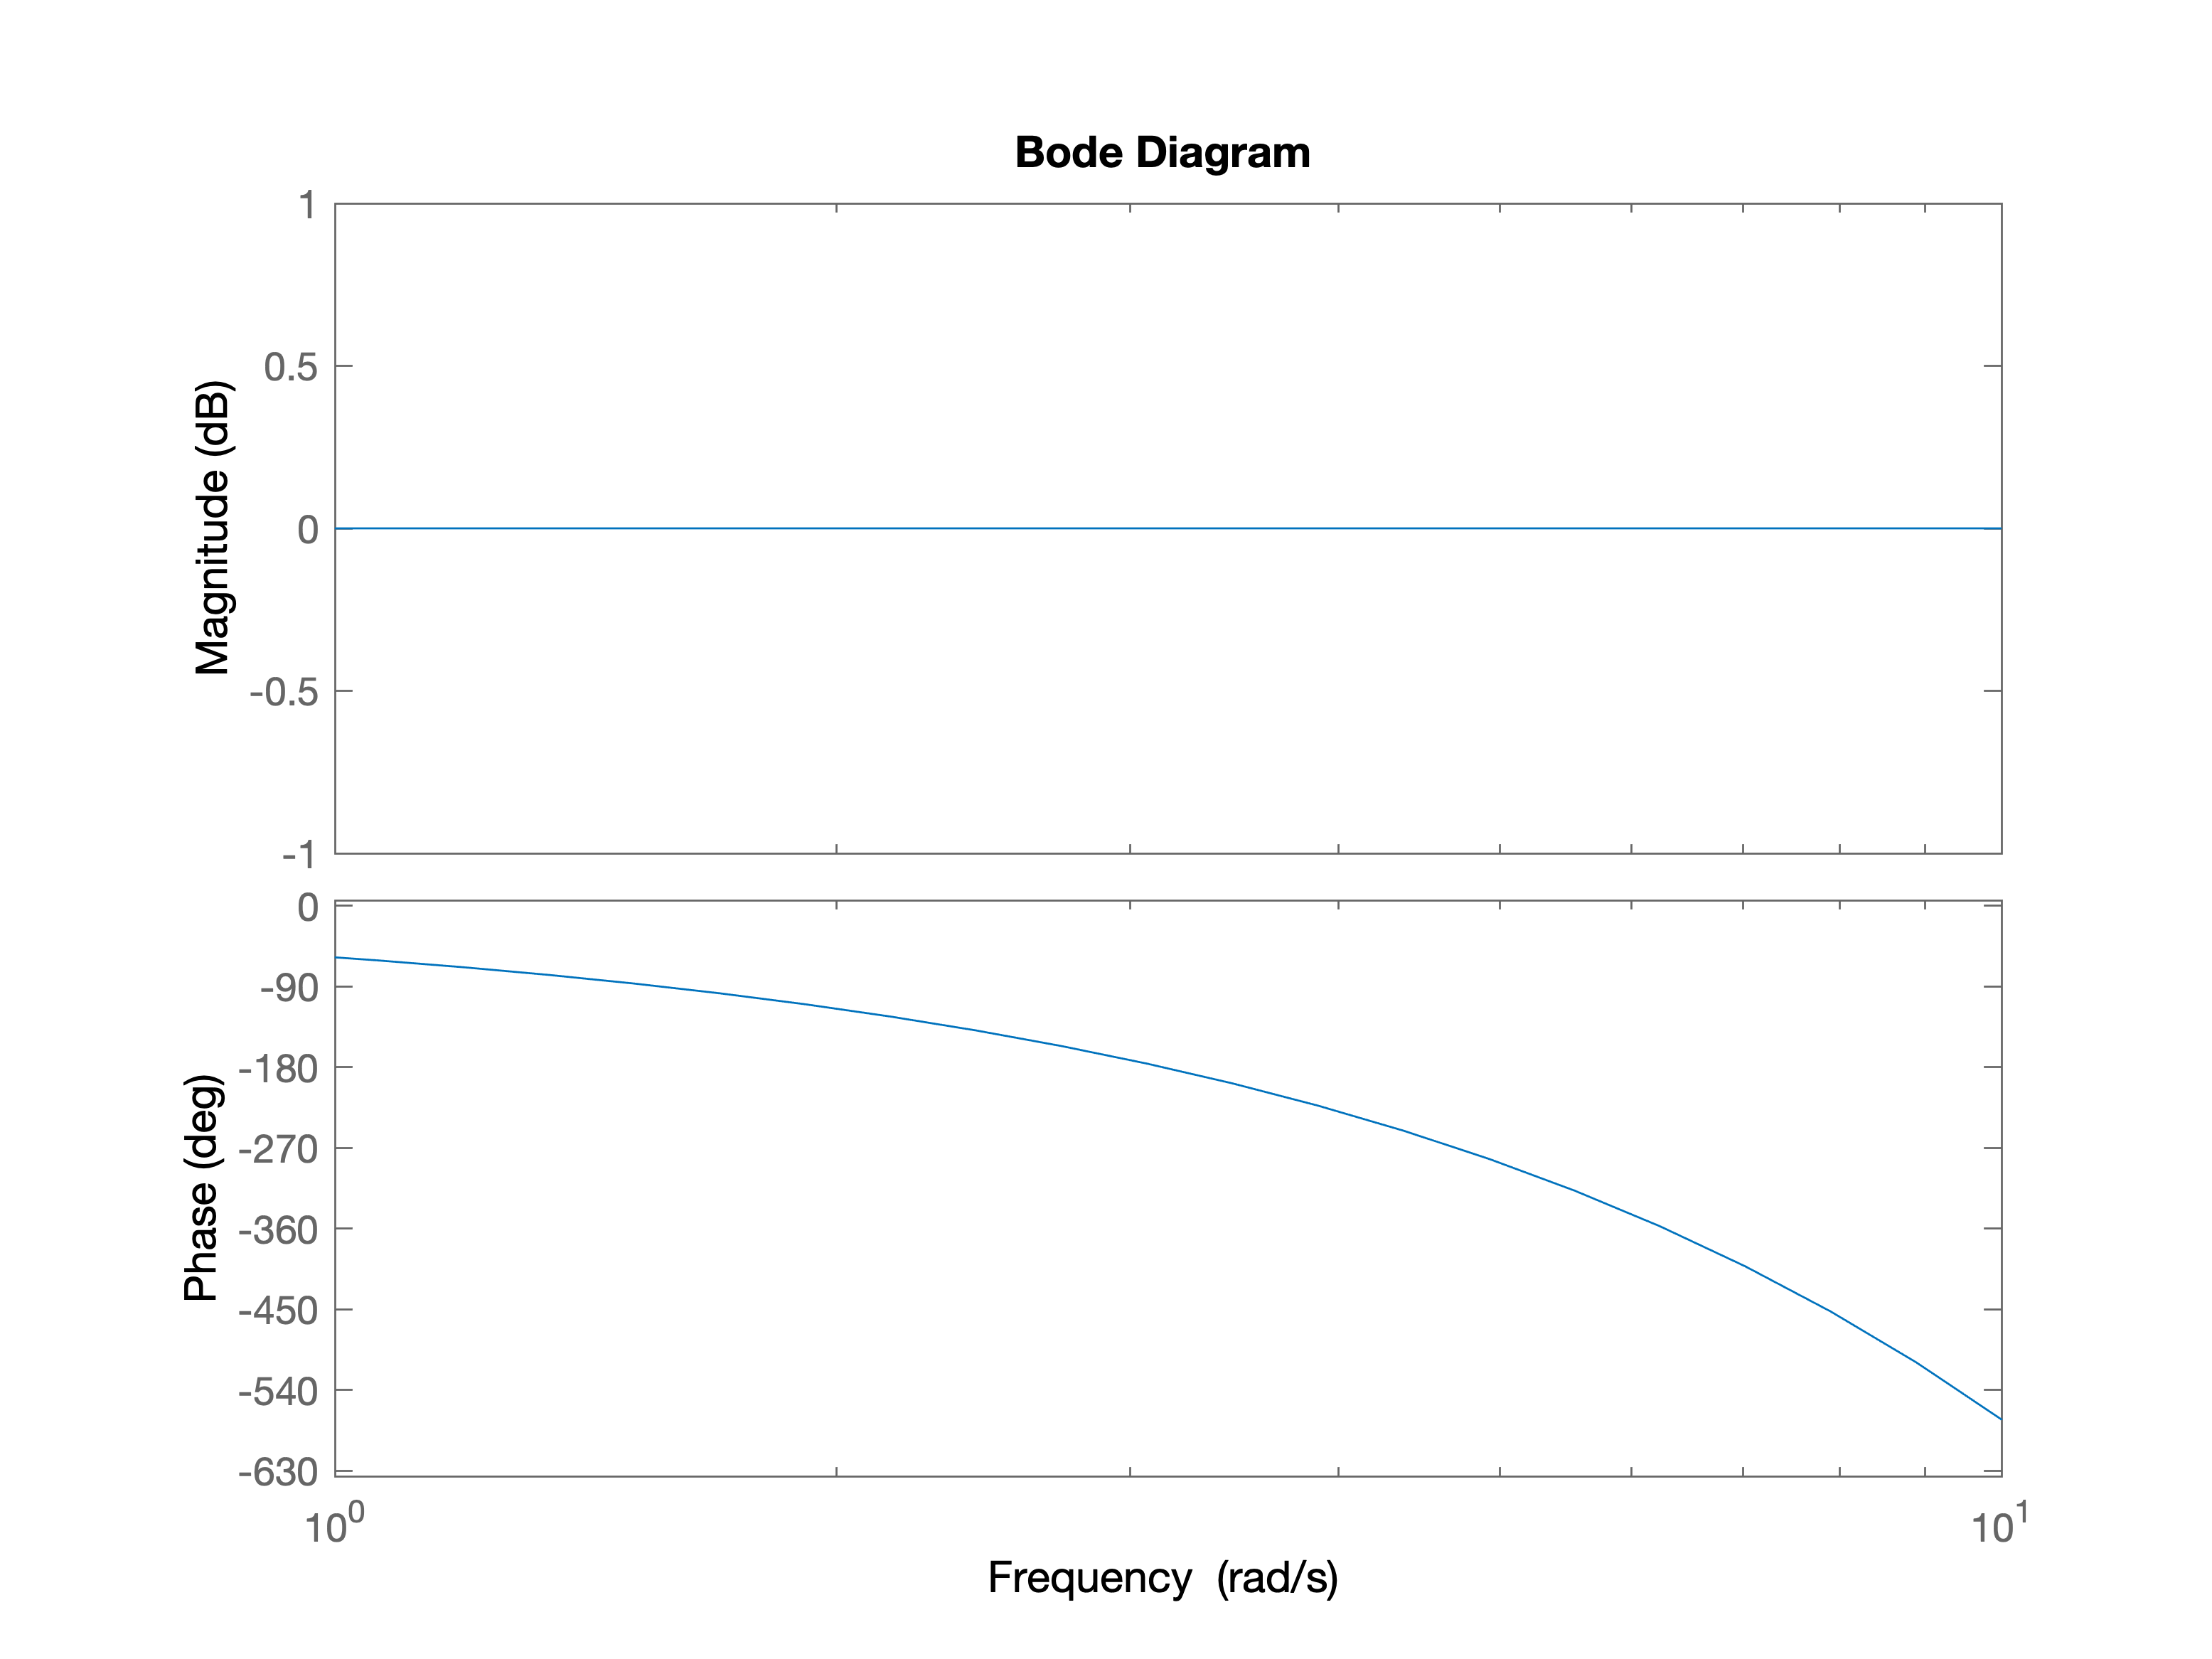
\includegraphics[width=12cm]{../Figure/Q1/bode.png}
\end{figure}

There is no pole in imaginary axis and nyquist path is from $0 \to \infty \to -\infty\to 0$.
\begin{figure}[H]
	\caption{Closed contour in the s plane}
	\centering
	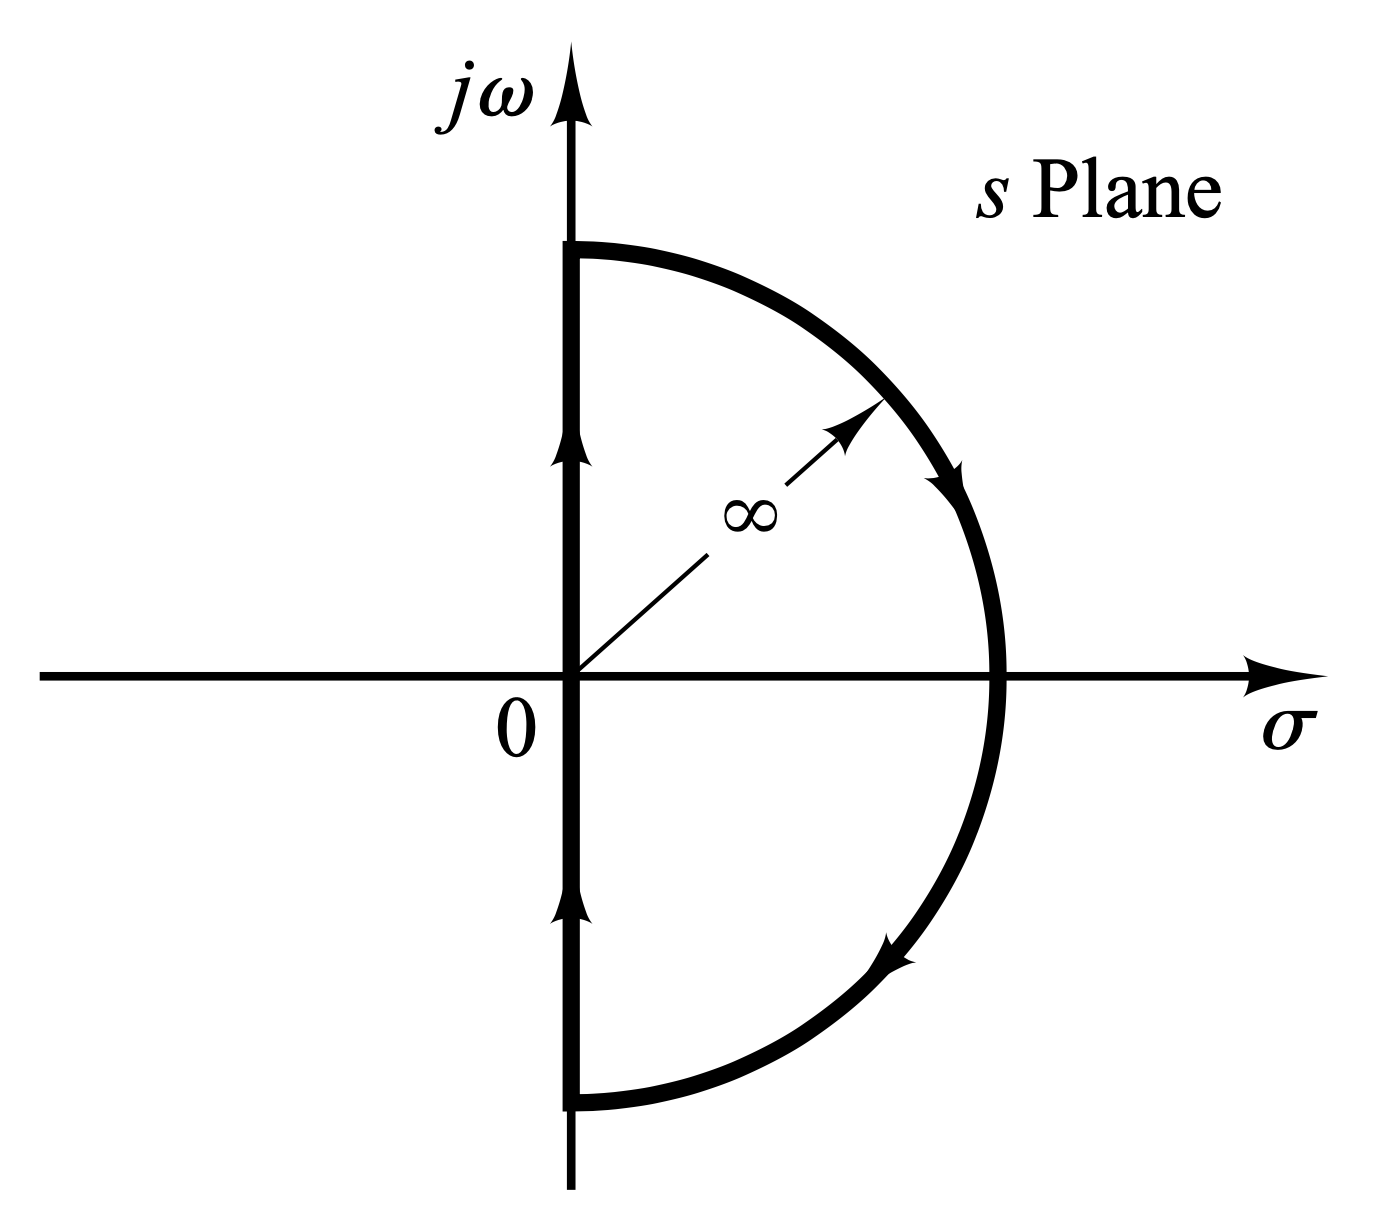
\includegraphics[width=12cm]{../Figure/Q1/Nyquist_path.png}
\end{figure}
So the Nyquist plot is circle in orogin with radius 1 and clock wise.
\begin{figure}[H]
	\caption{Nyquist plot using MATLAB ($\tau = 1$)}
	\centering
	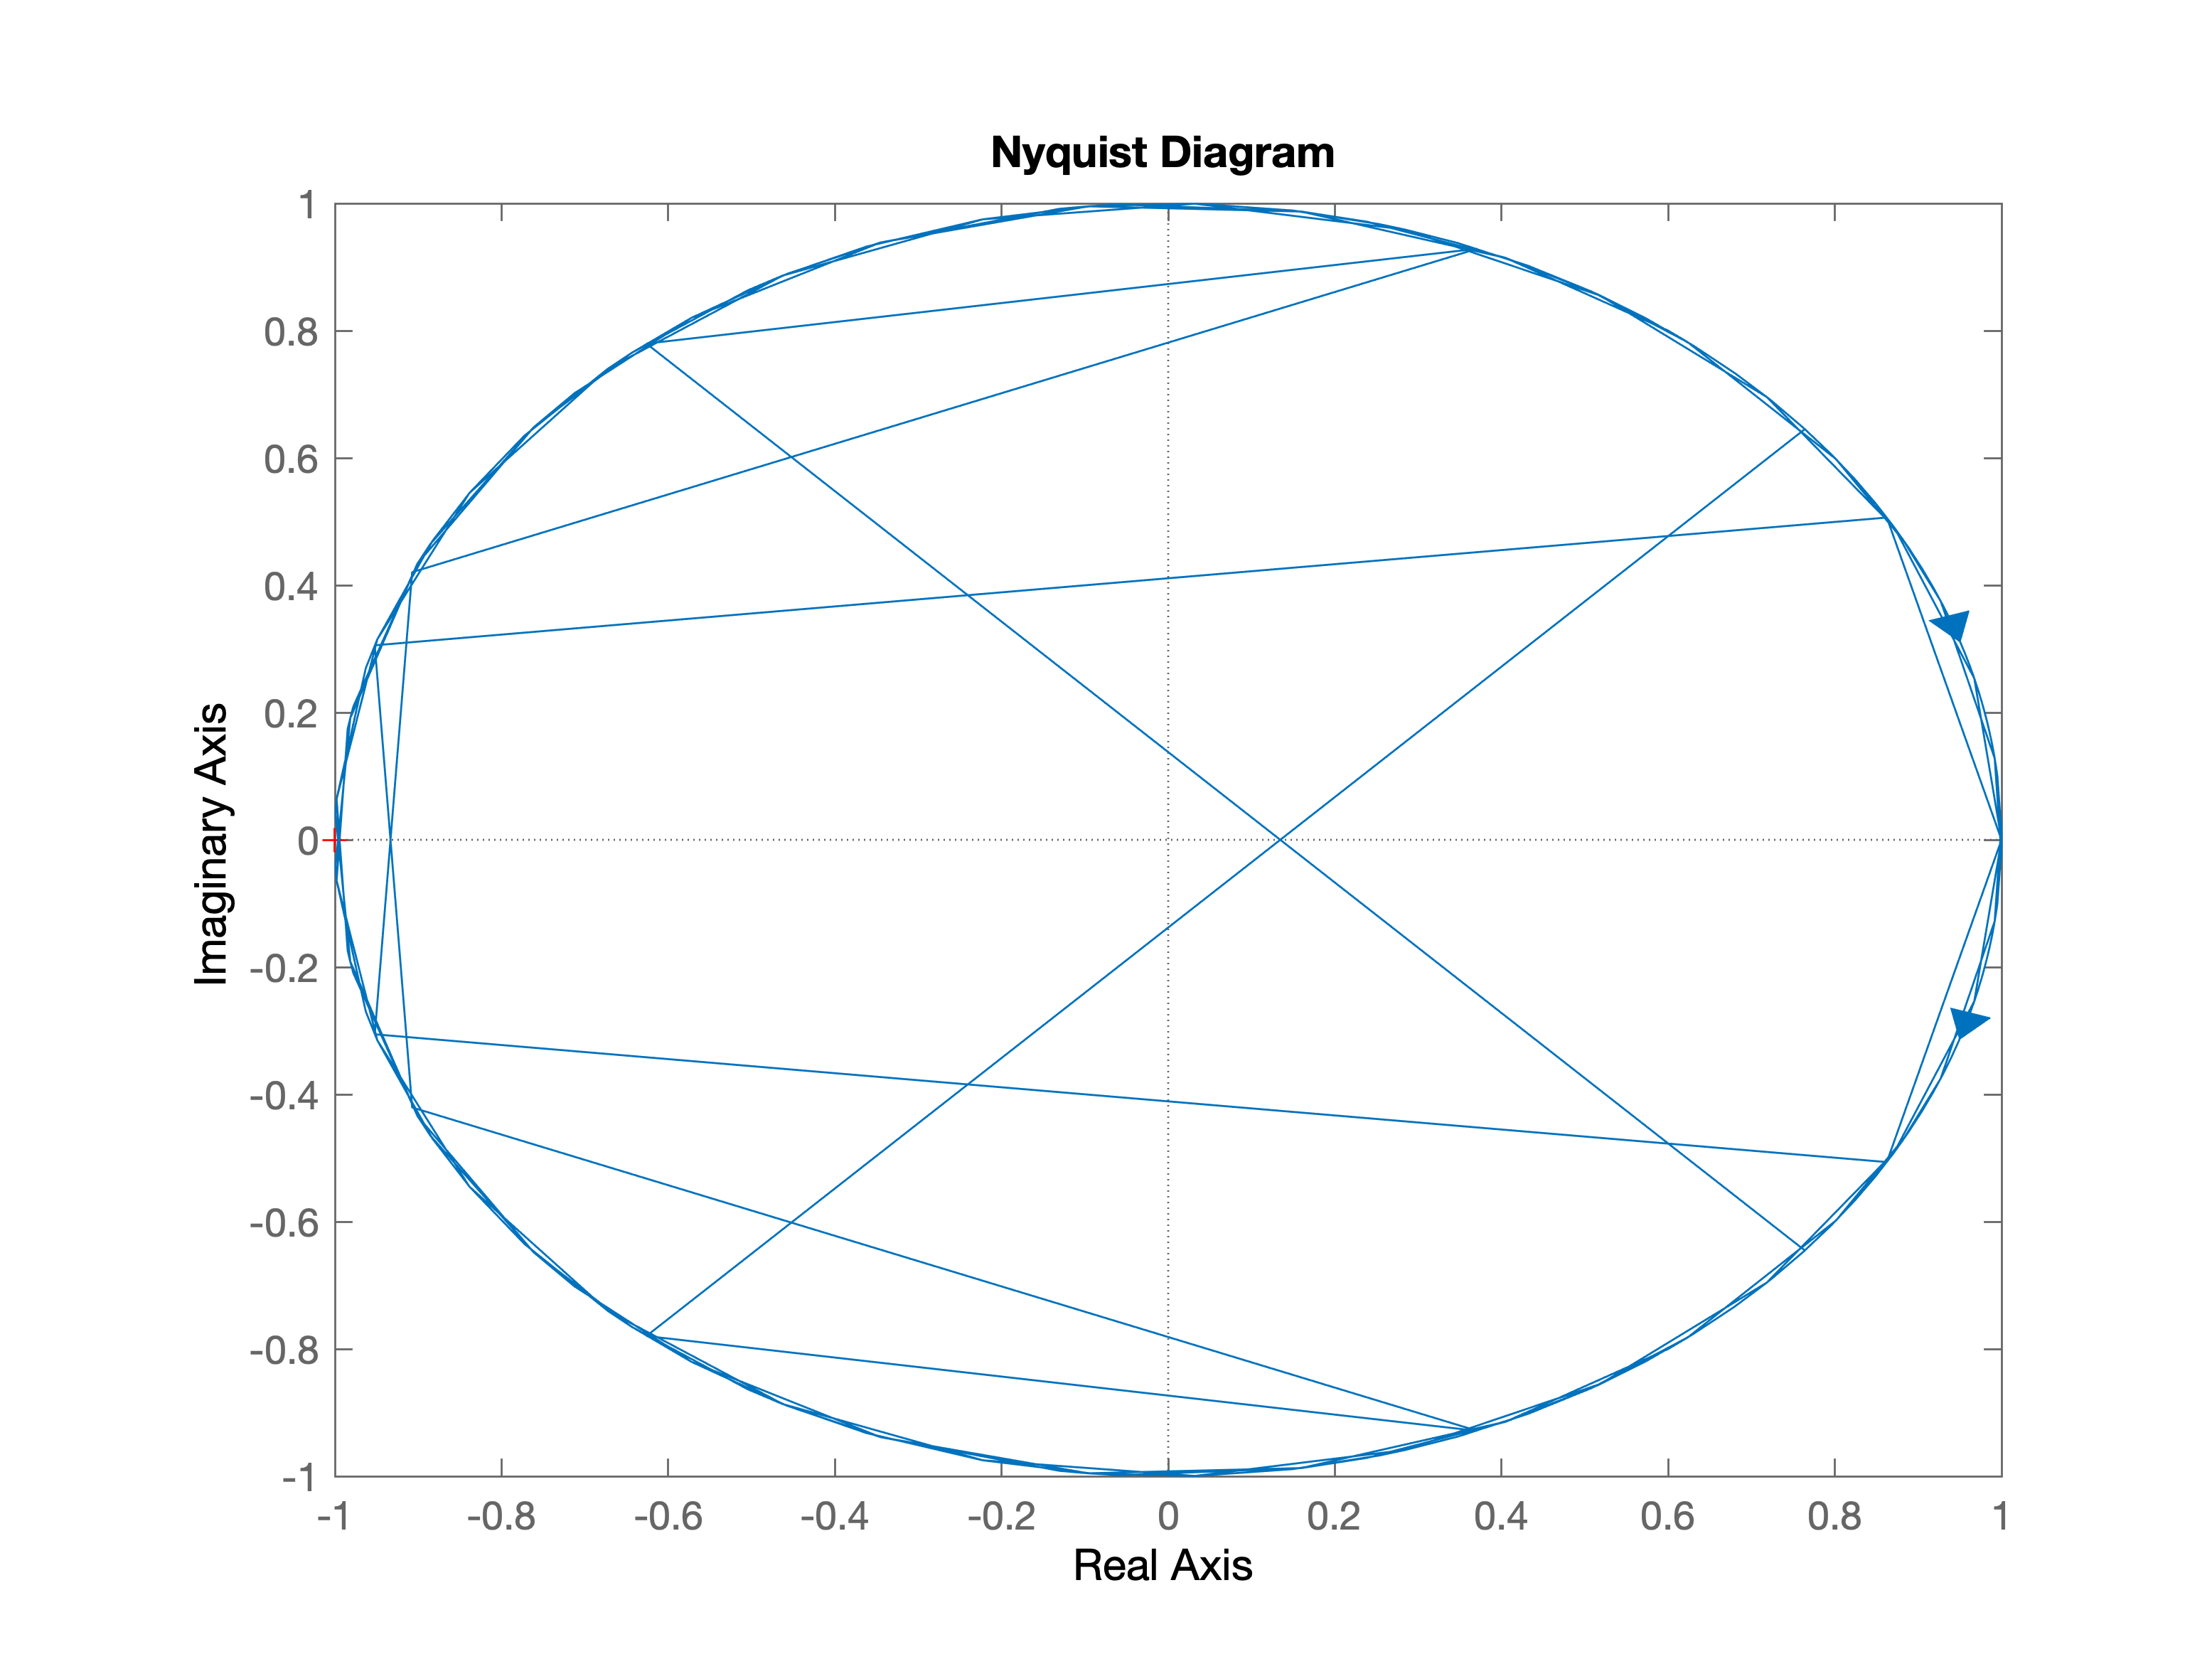
\includegraphics[width=12cm]{../Figure/Q1/nyquist.png}
\end{figure}
